\documentclass{article}
\usepackage{amsmath,amstext,amssymb}
\usepackage[ttscale=0.6]{libertine}
\usepackage[libertine]{newtxmath}
\usepackage{siunitx}
\usepackage{inconsolata}
\usepackage{wrapfig}

\usepackage{sectsty}
\allsectionsfont{\sffamily}

\usepackage{xcolor}
\usepackage[colorlinks=true,
            linkcolor=blue,
            urlcolor=blue,
            breaklinks,
            pdftex,
            allbordercolors=white]{hyperref}
\usepackage{graphicx}
\usepackage{booktabs}
\usepackage[version=4]{mhchem}
\usepackage{parskip}

\usepackage{datetime2}
\renewcommand{\DTMdisplaydate}[4]{#1-#2-#3}

\begin{document}

\begin{center}
    \Large{\textbf{\sffamily{Setting Up THAMES v2.5 Input}}}
\end{center}
\begin{center}
    \large{Jeffrey W. Bullard\footnote{Special thanks to Dr. Dmitrii Kulik who
    provided invaluable guidance for building GEMS3K and GEM-Selektor.}}
\end{center}
\begin{center}
    \large{\DTMnow}
\end{center}

\vspace{0.25truein}
\tableofcontents

\vspace{0.25truein}
This document provides guidance on how to build THAMES on an Apple computer running
Mac OS.  Very similar instructions should apply to Windows and especially to Linux
computers.  The build process from scratch is somewhat complicated due to the need
to build and install the GEMS3K standalone library and the GEM-Selektor software.

\section{Software Requirements}
The following software must be installed and running properly on your computer to
build and install all the components:
\begin{itemize}
    \item Git software versioning system.
    \item Cmake version 3.0 or later.
    \item A C++11 compiler.  This document will assume the Gnu C/C++ compiler suite with
        full support for C++11.
    \item Doxygen version 1.18.13 or later. This is needed only for generating the
        documentation.
    \item (Optional) \LaTeX typesetting software.  This is needed only for building the PDF versions
        of the documentation.  A recent installation of \TeX Live will suffice. 
    \item (For Linux) The packages build-essentials, libx11-xcb-dev, and libglu1-mesa-dev.
        These can be installed on Linux using a command like \verb!sudo apt-get install build-essentials!.  On Mac OS, the first two should not need to be installed, but mesa can be
        installed using Macports or Homebrew, for example \verb!sudo port install mesa! when
        using Macports.
\end{itemize}
This document will assume that all of these packages have been installed already.

\section{Downloading the Software}
Create a working directory somewhere in your home path.  For this document, the working
directory will be called \verb!$WORKDIR!.  You should substitute to the path to your working
directory everywhere you see that.

The remainder of these instructions require that you enter commands on the command line
(the Terminal app on Mac OS, for example).  These commands will be typeset in monospace
font to distinguish them from other instructions.

\subsection{GEMS3K Standalone Library}
\begin{enumerate}
        \item \verb!cd $WORKDIR!
        \item \verb!mkdir gitGEMS!
        \item \verb!cd gitGEMS!
        \item \verb!mkdir standalone!
        \item \verb!cd standalone!
        \item \verb!git clone https://bitbucket.org/gems4/gems3k.git .!
\end{enumerate}

\subsection{GEM-Selektor}
\begin{enumerate}
        \item \verb!cd $WORKDIR/gitGEMS!
        \item \verb!mkdir GEMS3GUI!
        \item \verb!cd GEMS3GUI!
        \item \verb!git clone https://bitbucket.org/gems4/gems3gui.git .!
\end{enumerate}

\subsection{THAMES 2.5}
If you already have THAMES installed from github and you want to keep any local changes you
have made, then go to the directory where
you installed it and execute these commands:
\begin{enumerate}
    \item git stash
    \item git pull
\end{enumerate}
The first command stashes away your local changes so they won't be lost.  The second
command pulls all the updates from the remote repository.  Later, if you want to
put your local changes back into the updated version, you can run the command
\verb!git stash pop!

On the other hand, if you have never installed THAMES on your computer, then
follow these steps:
\begin{enumerate}
        \item \verb!cd $WORKDIR!
        \item \verb!mkdir THAMES!
        \item \verb!cd THAMES!
        \item \verb!git clone https://github.tamu.edu/jwbullard/THAMES.git .!
\end{enumerate}

\subsection{Qt}
\begin{enumerate}
    \item \verb!cd $WORKDIR!
    \item \verb!mkdir Qt!
    \item Download the Qt software version 5.12.5 (community) for Gnu C++ from 
        \href{https://qt.io}{https://qt.io} into the Qt directory you just made.
        Use the settings shown in the figure.
\end{enumerate}

\begin{center}
    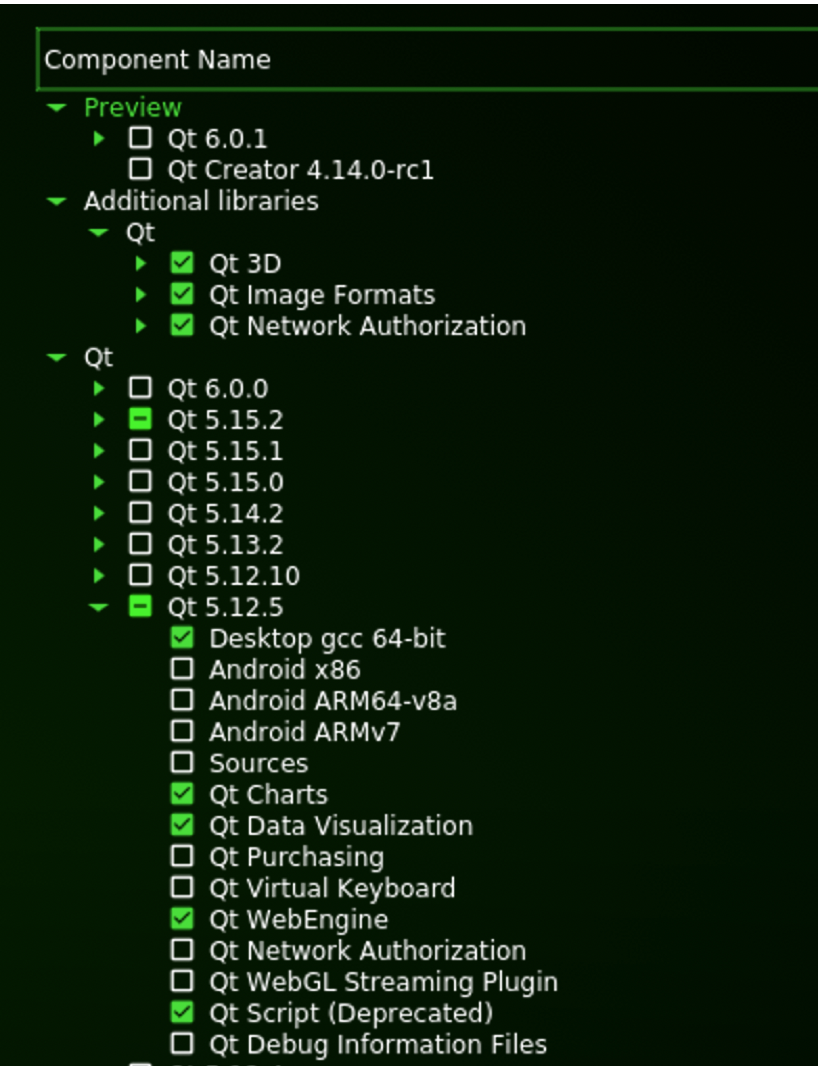
\includegraphics[scale=0.4]{Figures/Qt-screen.png}
\end{center}

\section{Build and Install GEMS3K Standalone Library}
First, there is one tweak that must be made to the downloaded version of GEMS3K.
You can apply that tweak with the following command:
\begin{enumerate}
    \item \verb!/bin/cp $WORKDIR/THAMES/src/GEMS3K-mods/node.h $WORKDIR/gitGEMS/standalone/GEMS3K/.!
\end{enumerate}

If you have administrator privileges on your computer (Mac or Linux), then these commands
will install the library:
\begin{enumerate}
        \item \verb!cd $WORKDIR/gitGEMS/standalone!
        \item \verb!sudo ./install.sh!
\end{enumerate}
If you do not have administrator privileges, then you will need to work with your IT
help desk to get this installed.

\section{Build and Install GEM-Selektor}
Start up Qt.  On Linux, the Qt executable is in \verb!$WORKDIR/Qt/Tools/QtCreator/bin/!
On a Mac, it is easiest to just use the Finder, navigate to \verb!$WORKDIR/Qt!, and then
double-click on the ``Qt Creator'' app.

From within the QtCreator Software, open the project \verb!$WORKDIR/gitGEMS/GEMS3GUI/gems3gui.pro!.
This step may take some time to complete.  The progress will be shown in a small window.  Wait
until it is finished.

Click on the Build item in the sidebar to set the Build settings as shown in the figure:

\begin{center}
    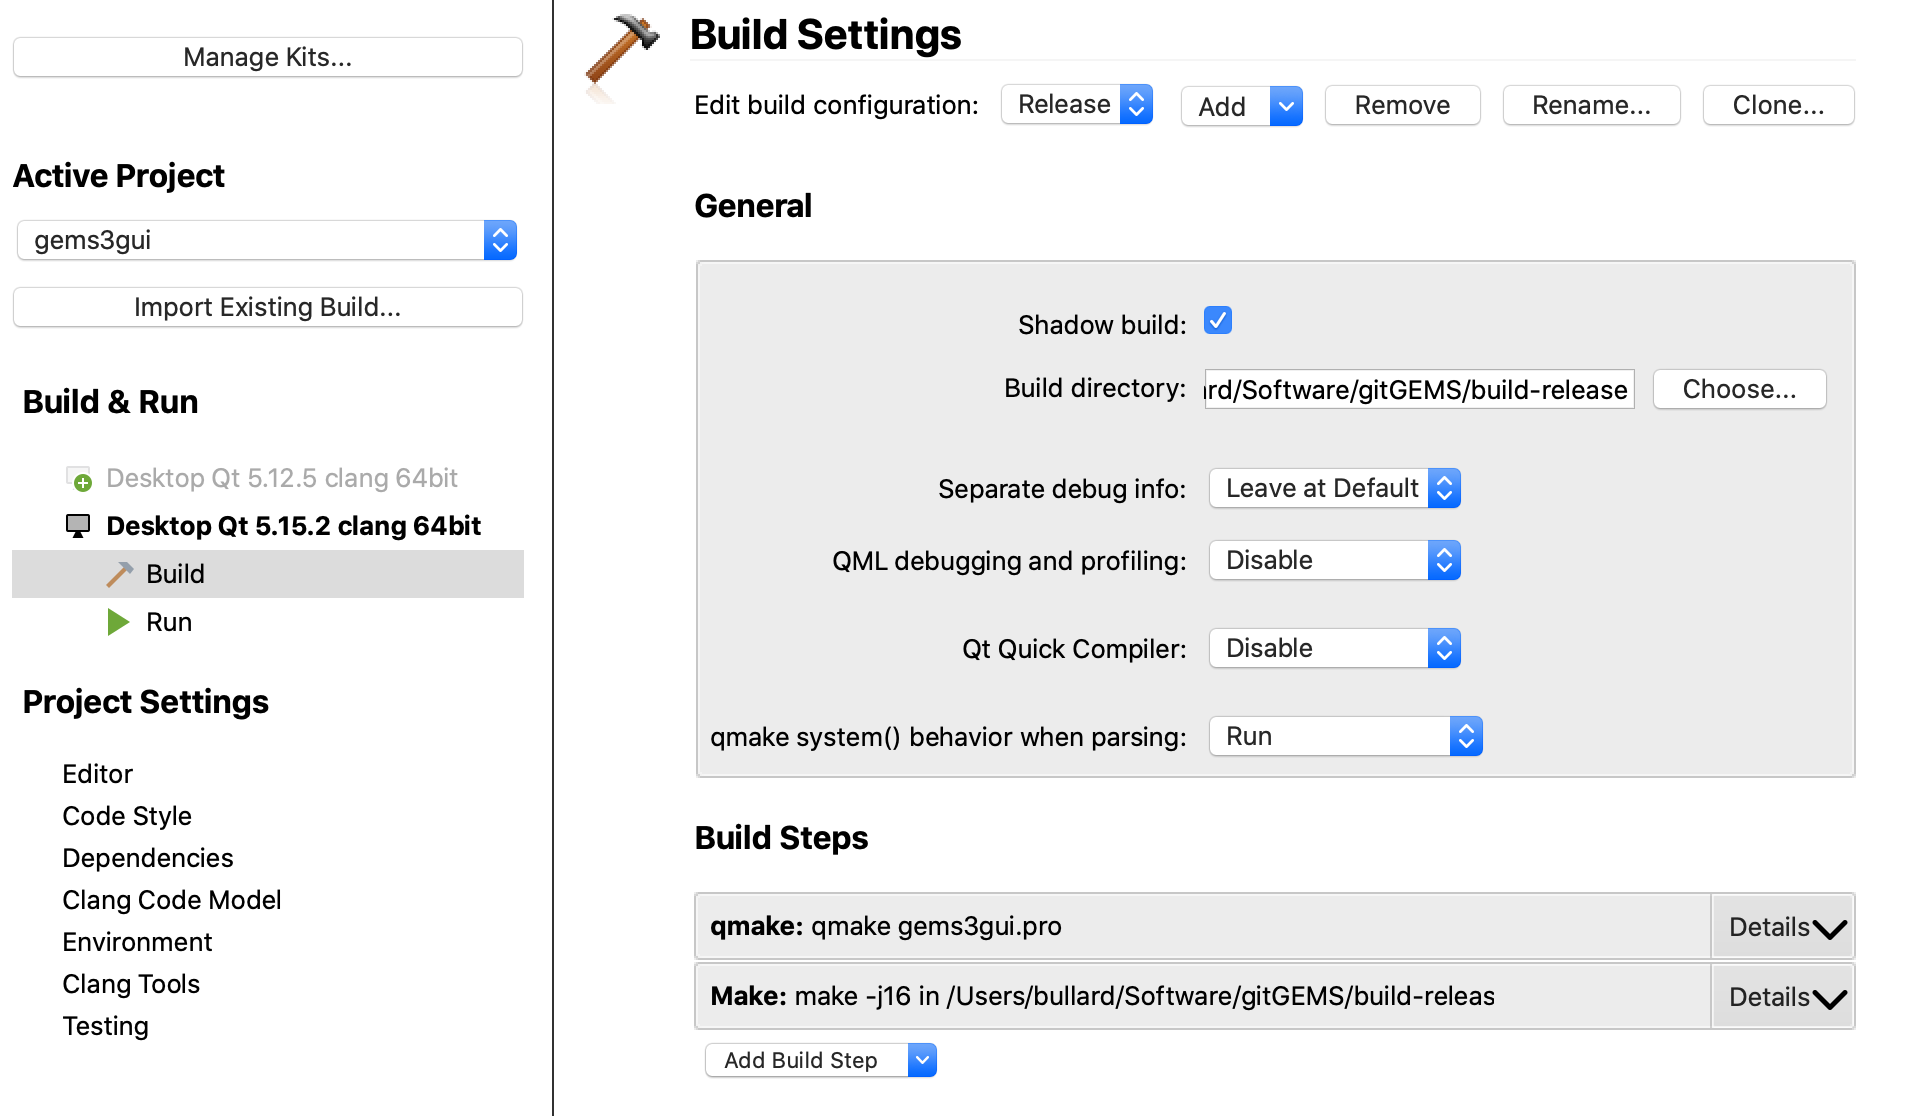
\includegraphics[width=0.8\textwidth]{Figures/Qt-build-settings.png}
\end{center}

Next, click on the Run item in the sidebar to set the Runtime settings as shown in the figure:

\begin{center}
    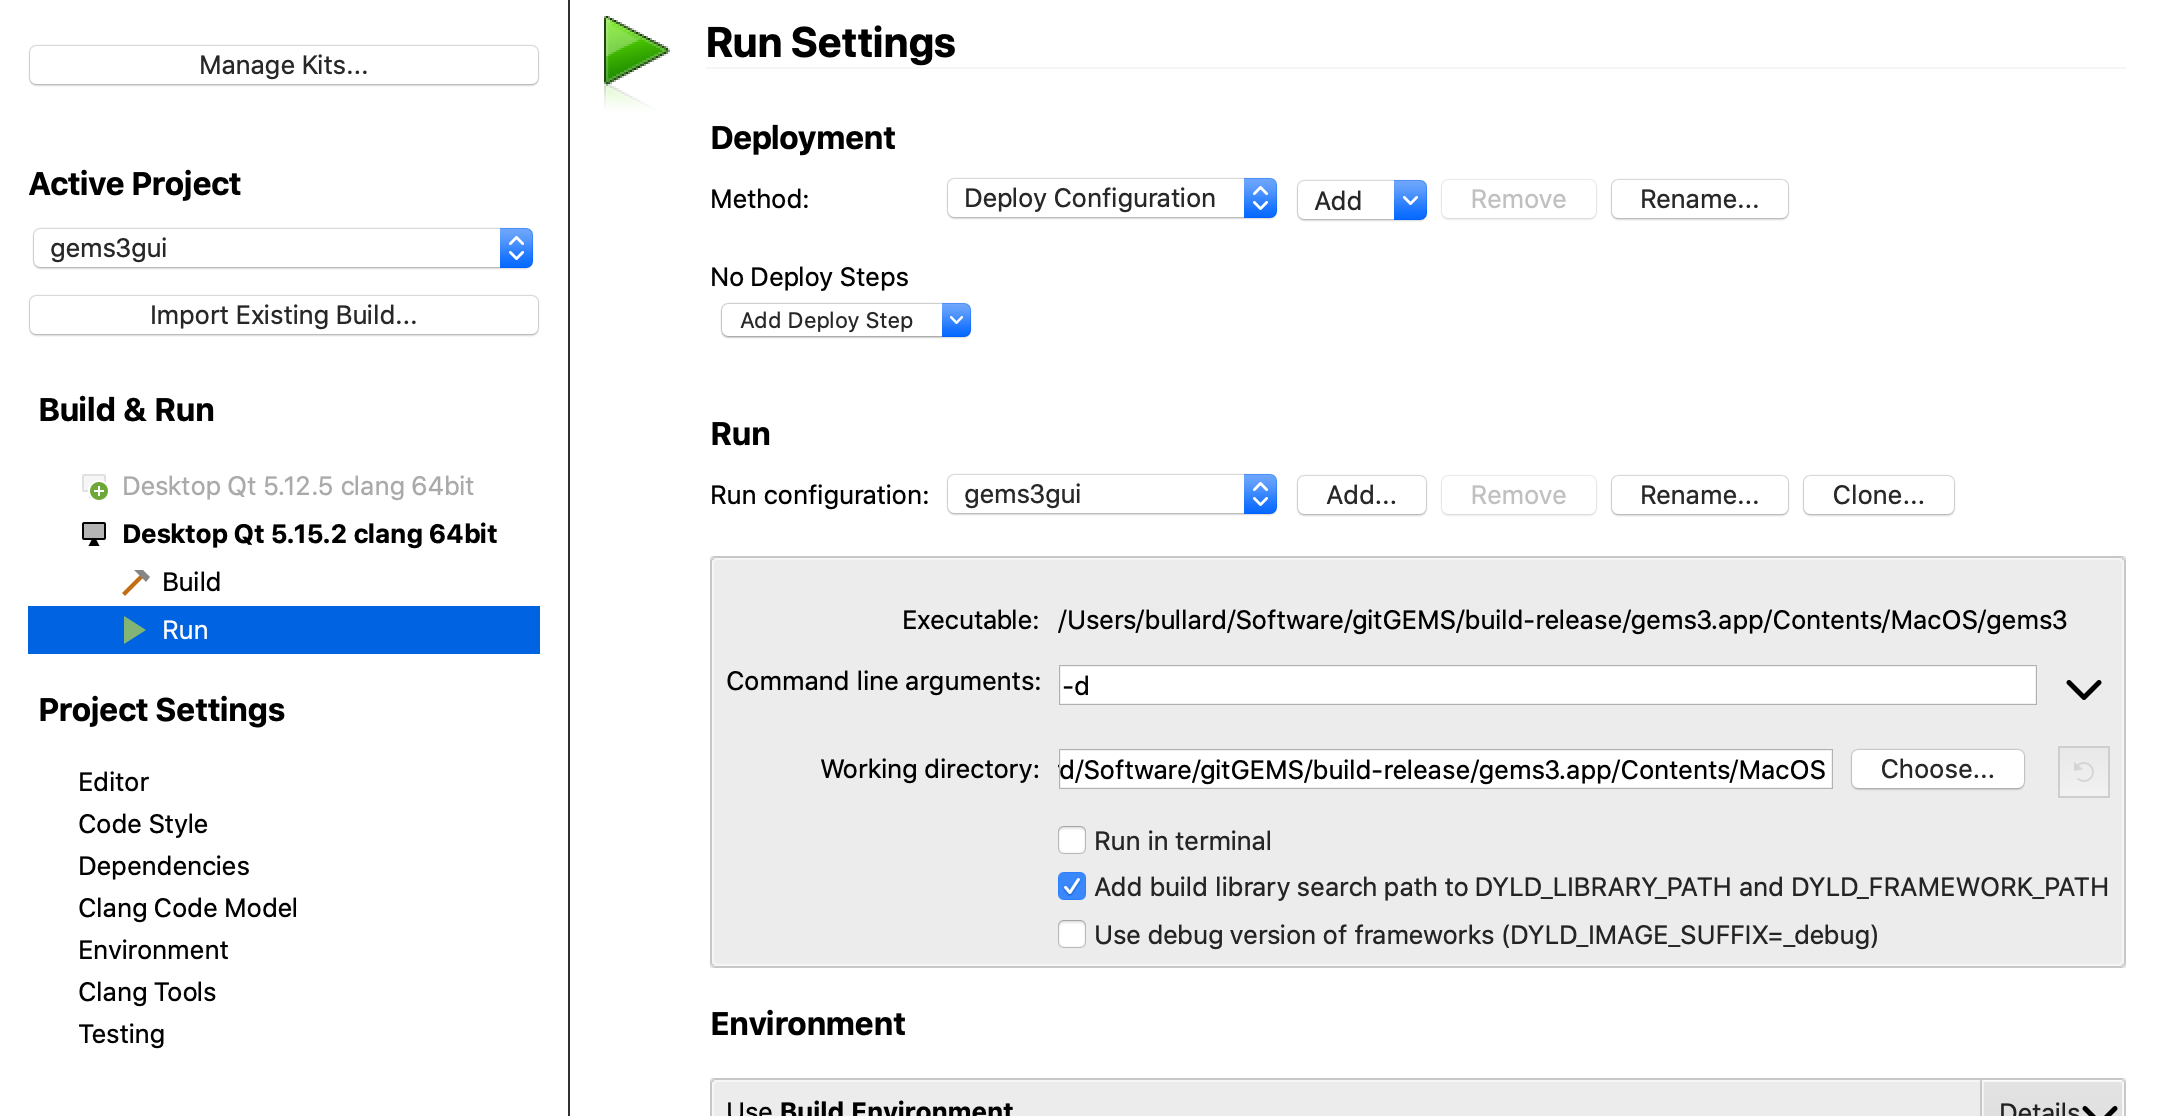
\includegraphics[width=0.8\textwidth]{Figures/Qt-run-settings.png}
\end{center}

Next, build the GEM-Selektor from within Qt by clicking on the Build icon (looks like a hammer).
This could take a while to build.  When it is finished, check the output log to make sure there
are no fatal errors.  Multiple warnings are okay, though.  If you configured the build settings
correctly, this build step will create a new directory, \verb!$WORKDIR/gitGEMS/build-release!

\subsection{One Extra Step for a Mac}
On a Mac, you now need to go to the command line and run this command:
\begin{verbatim}
/bin/cp -R $WORKDIR/gitGEMS/GEMS3GUI/Resources \\
    $WORKDIR/gitGEMS/build-release/Contents/gems3.app/Contents/.
\end{verbatim}

\subsection{Install Third-Party Data Repositories}
Make sure that GEM-Selektor is not running for this step.
Any third-party thermodynamic databases, such as Cemdata18 or Mines, should be copied into
their new location, which is
\begin{verbatim}
$WORKDIR/gitGEMS/build-release/gems3.app/Contents/Resources/DB.default
\end{verbatim}

If you have a previous version of GEM-Selektor installed on your computer with
the third-party libraries already there, you can just copy the contents of your old
DB.default directory to this new location.

\subsection{Test GEM-Selektor}
You should now be able to run GEM-Selektor from within Qt by clicking on the Run icon (looks
like a green triangle pointing to the right). 

\section{Build and Install THAMES}
If all the previous steps have been executed successfully, installing THAMES should be pretty
straightforward.
\begin{enumerate}
    \item \verb!cd $WORKDIR/THAMES/build!
    \item \verb!cmake ..!
    \item \verb!make!
    \item \verb!make install!
\end{enumerate}
The last step will put the thames and vcctl2thames executables into the directory
\begin{verbatim}
$WORKDIR/THAMES/bin
\end{verbatim}
\end{document}
